\documentclass[10pt, a4paper,spanish]{article}

\usepackage{mystyle}
\usepackage{myvars}



%-----------------------------

\begin{document}

	\maketitle % Insert title

	\thispagestyle{fancy} % All pages have headers and footers


%-----------------------------
%	ABSTRACT
%-----------------------------

	\begin{abstract}
		\noindent En este documento se analiza el comportamiento de los algoritmos de generación de árboles de decisión \emph{ID3} y \emph{J48} desde el punto de vista de la discretización de atributos (en el caso de \emph{ID3} de forma manual). Para ello se ha utilizado el conjunto de datos \emph{Thoracic Surgery Data Data Set}\cite{dataset:thoracic}. La herramienta utilizada para el aprendizaje automático ha sido \emph{WEKA}\cite{tool:weka}. La metodología experimental que se ha seguido a lo largo del documento ha sido un \emph{Hold-Out} de $\frac{1}{3}$ para tareas de prueba.
	\end{abstract}

%-----------------------------
%	TEXT
%-----------------------------


	\section{¿Por qué no se puede aplicar directamente ID3?}

		\paragraph{}
		El conjunto de datos utilizado\cite{dataset:thoracic} está formado por \textbf{470} instancias, las cuales describen resultados acerca de la esperanza de vida tras operaciones de cáncer pulmonar. Dicho conjunto presenta atributos con las siguientes características:
		\begin{itemize}
			\setlength\itemsep{0em}
			\item 10 atributos de tipo categórico binario.
			\item 1 atributo de tipo categórico con 3 valores distintos.
			\item 1 atributo de tipo categórico con 4 valores distintos.
			\item 1 atributo de tipo categórico con 7 valores distintos.
			\item 1 atributo de tipo numérico real en el rango $[1.44, 6.3]$.
			\item 1 atributo de tipo numérico real en el rango $[0.96, 86.3]$.
			\item 1 atributo de tipo numérico entero en el rango $[21, 87]$.
			\item 1 atributo de tipo categórico binario, que representa el valor de la clase.
		\end{itemize}

		\paragraph{}
		La razón por la cual no se puede aplicar el algoritmo \emph{ID3} sobre el mismo es la existencia de atributos de naturaleza numérica, para los cuales dicho algoritmo no está diseñado. Por lo tanto, para que la clasificación con este algoritmo pueda llevarse a cabo, será necesaria una tarea de adaptación previa del conjunto de datos a los requisito de \emph{ID3}

	\section{Realice las modificaciones previas en el fichero de datos para que pueda llevar a cabo lo anterior y proporcione los resultados aplicando el método de retención o Hold-Out para la formación del experimento}

		\paragraph{}
		Para poder aplicar el algoritmo \emph{ID3} existen distintas alternativas, entre ellas se encuentran la discretización de los atributos numéricos o la eliminación de los mismos. Nótese que la eliminación no es la mejor alternativa en la mayoría de casos, debido a que de esta manera se deja de utilizar información valiosa para la tarea de clasificación. Por tanto, en este caso se ha decidido realizar una discretización.

		\paragraph{}
		El método que se ha utilizado para dicha tarea ha sido el más básico posible, realizando una partición en \textbf{4 intervalos de la misma anchura} sobre el rango de valores que toma cada uno de los atributos numéricos. Tras procesar el conjunto de datos con el algoritmo \emph{ID3} teniendo en cuenta la metodología experimental citada anteriormente, el árbol de decisión generado se ilustra en la figura \ref{fig:id3-tree}. Tal y como se puede apreciar, este árbol presenta muchas ramificaciones. La causa de ello es que por cada atributo numérico, se han generado 4 ramas y dado que \emph{ID3} genera todas las posibles combinaciones posibles a partir de las instancias destinadas a la fase de entrenamiento, el fenómeno combinatorio produce dicho efecto.

		\begin{figure}[h]
			\begin{center}
				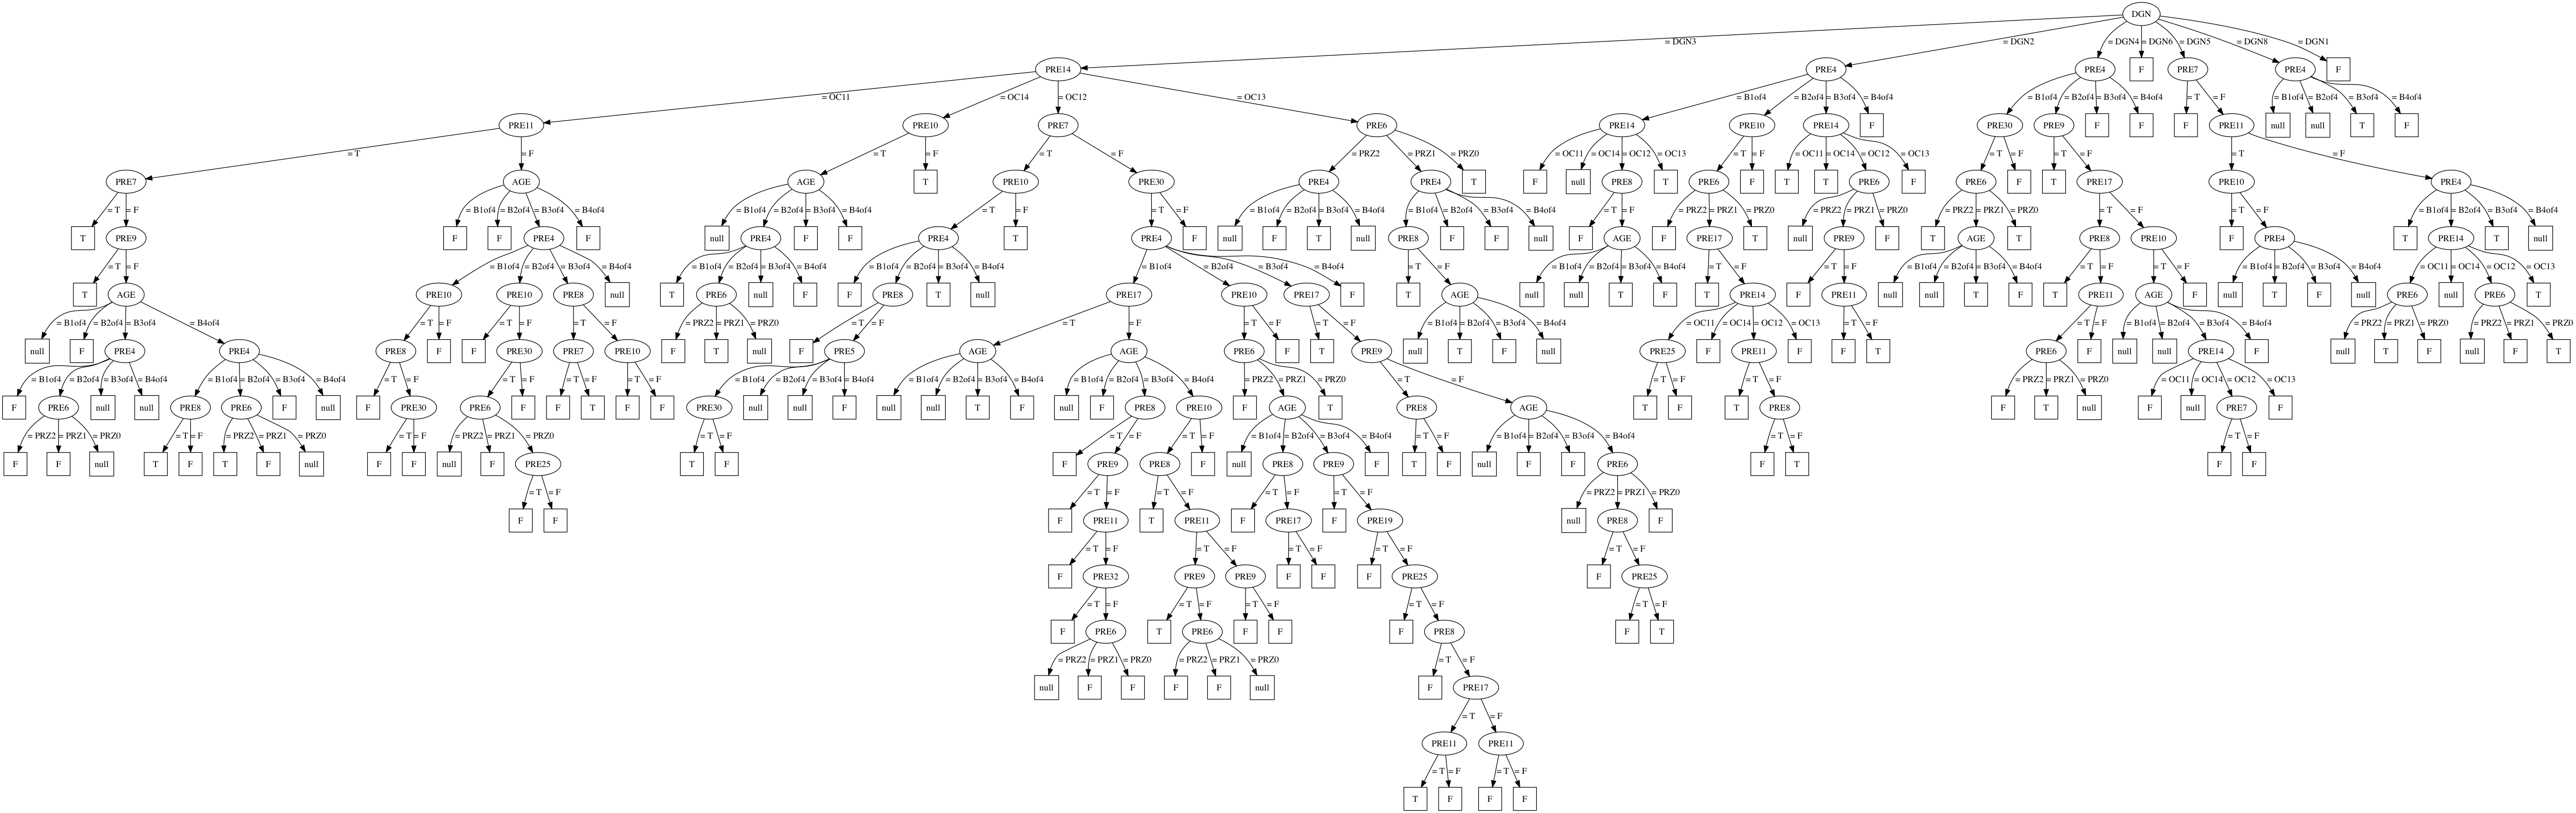
\includegraphics[width=\textwidth]{id3-tree}
			\end{center}
			\caption{Árbol de decisión generado a partir del algoritmo \emph{ID3}}
			\label{fig:id3-tree}
		\end{figure}

		\paragraph{}
		La matriz de confusión resultante de dicha clasificación se muestra en la tabla \ref{table:confusion-matrix-id3}. Nótese que se han utilizado \textbf{160 instancias} pero el árbol de decisión ha dejado sin clasificar $5$ de ellas, por lo que la tasa de acierto global es del $72.5\%$.

		\begin{table}[h]
			\begin{center}
				\begin{tabular}{r c c|c|l}
					& & \multicolumn{2}{ c }{Valor Real} \\ \cline{3-4}
					& & \multicolumn{1}{ |c| }{Positivo} & \multicolumn{1}{ |c| }{Negativo} & \multicolumn{1}{ l }{$p_j$}\\ \cline{2-4}
					\multicolumn{1}{  c  }{\multirow{2}{*}{Valor Predicho} } 	& \multicolumn{1}{ |c| }{Positivo} & $5$ & $18$ &  $0.2173$   \\ \cline{2-4}
					\multicolumn{1}{  c  }{}                        					& \multicolumn{1}{ |c| }{Negativo} & $21$  & $111$ & $0.8409$ \\ \cline{2-4}
					& \multicolumn{1}{ c }{$\pi_j$} & \multicolumn{1}{ c }{$0.1677$} & \multicolumn{1}{ c }{$0.8322$} & \multicolumn{1}{ l }{$N = 155$}
				\end{tabular}
			\end{center}
			\caption{Matriz de confusión del conjunto de datos discretizado previamente y después entrenado por el algortimo \emph{ID3}}
			\label{table:confusion-matrix-id3}
		\end{table}


	\section{Volviendo al fichero original, pase el algoritmo J48 también aplicando el método de retención o Hold-Out. Analice el árbol obtenido sin poda. ¿Se podría prescindir de algún atributo? Si es así, hágalo y compare los resultados de nuevo}

		\paragraph{}
		Puesto que el algoritmo \emph{J48} si que permite el procesado de conjunto de datos con atributos continuos, en este caso no es necesario realizar ninguna tarea previa para la generación del árbol de decisión. Utilizando la misma metodología de la sección anterior (Hold-Out de $1/3$) se obtiene el árbol de decisión de la figura \ref{fig:j48-tree-all}

		\begin{figure}[h]
			\begin{center}
				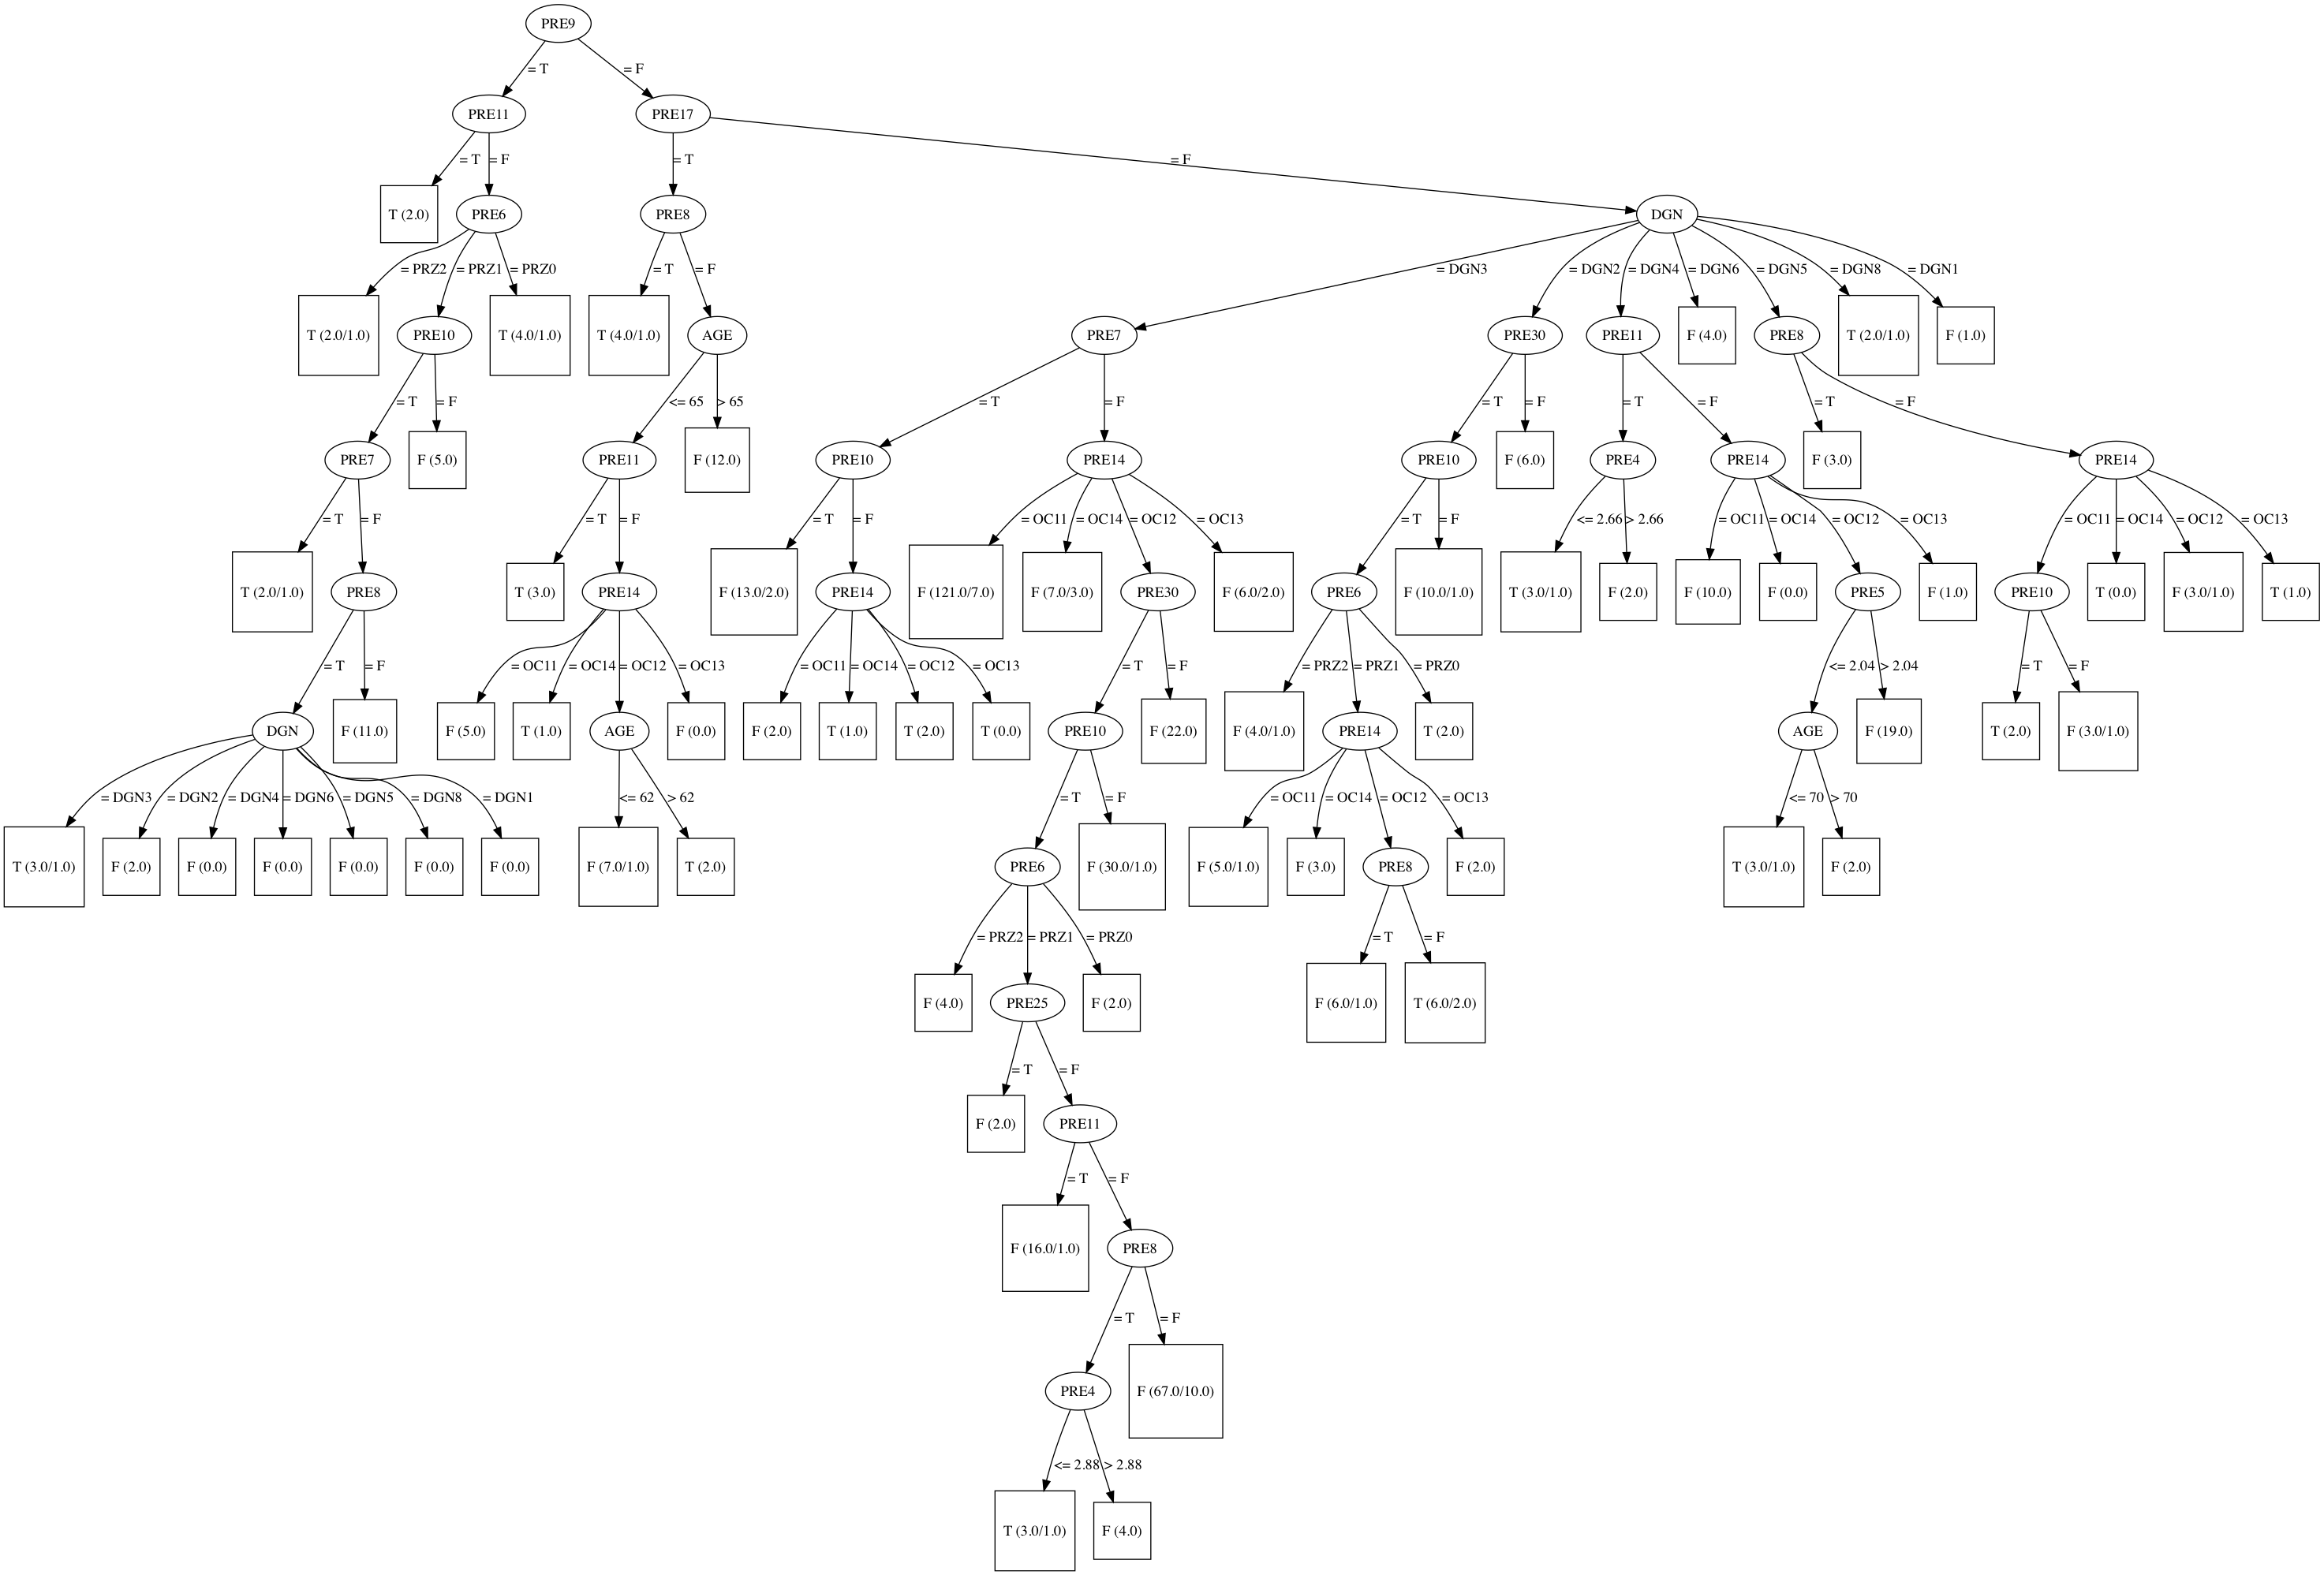
\includegraphics[width=\textwidth]{j48-tree-all}
			\end{center}
			\caption{Árbol de decisión generado a partir del algoritmo \emph{J48}}
			\label{fig:j48-tree-all}
		\end{figure}

		\paragraph{}
		Tras analizar el árbol se ha comprobado que $2$ de los atributos (\textbf{PRE19} y \textbf{PRE32}) no se han escogido para la construcción del árbol de decisión, por tanto, posteriormente se ha vuelto a generar a partir del algoritmo \emph{J48} otro árbol de decisión, pero esta vez eliminando del conjunto de datos dichos atributos. La matriz de confusión obtenida en con todos los atributos se muestra en la tabla \ref{table:confusion-matrix-j48-all}. La tasa de acierto resultante de dicha clasificación ha sido del $75\%$.

		\begin{table}[h]
			\begin{center}
				\begin{tabular}{r c c|c|l}
					& & \multicolumn{2}{ c }{Valor Real} \\ \cline{3-4}
					& & \multicolumn{1}{ |c| }{Positivo} & \multicolumn{1}{ |c| }{Negativo} & \multicolumn{1}{ l }{$p_j$}\\ \cline{2-4}
					\multicolumn{1}{  c  }{\multirow{2}{*}{Valor Predicho} } 	& \multicolumn{1}{ |c| }{Positivo} & $4$ & $18$ &  $0.1375$   \\ \cline{2-4}
					\multicolumn{1}{  c  }{}                        					& \multicolumn{1}{ |c| }{Negativo} & $22$  & $116$ & $0.8625$ \\ \cline{2-4}
					& \multicolumn{1}{ c }{$\pi_j$} & \multicolumn{1}{ c }{$0.1625$} & \multicolumn{1}{ c }{$0.8375$} & \multicolumn{1}{ l }{$N = 160$}
				\end{tabular}
			\end{center}
			\caption{Matriz de confusión del conjunto de datos entrenado por el algoritmo \emph{J48}}
			\label{table:confusion-matrix-j48-all}
		\end{table}

		\paragraph{}
		El árbol resultante de aplicar el algoritmo \emph{J48} eliminando los atributos \textbf{PRE19} y \textbf{PRE32} se muestra en la figura \ref{fig:j48-tree-some}. Además, en la tabla \ref{table:confusion-matrix-j48-all} se muestra la matriz de confusión, cuyos resultados son equivalentes al caso anterior.


		\begin{figure}[h]
			\begin{center}
				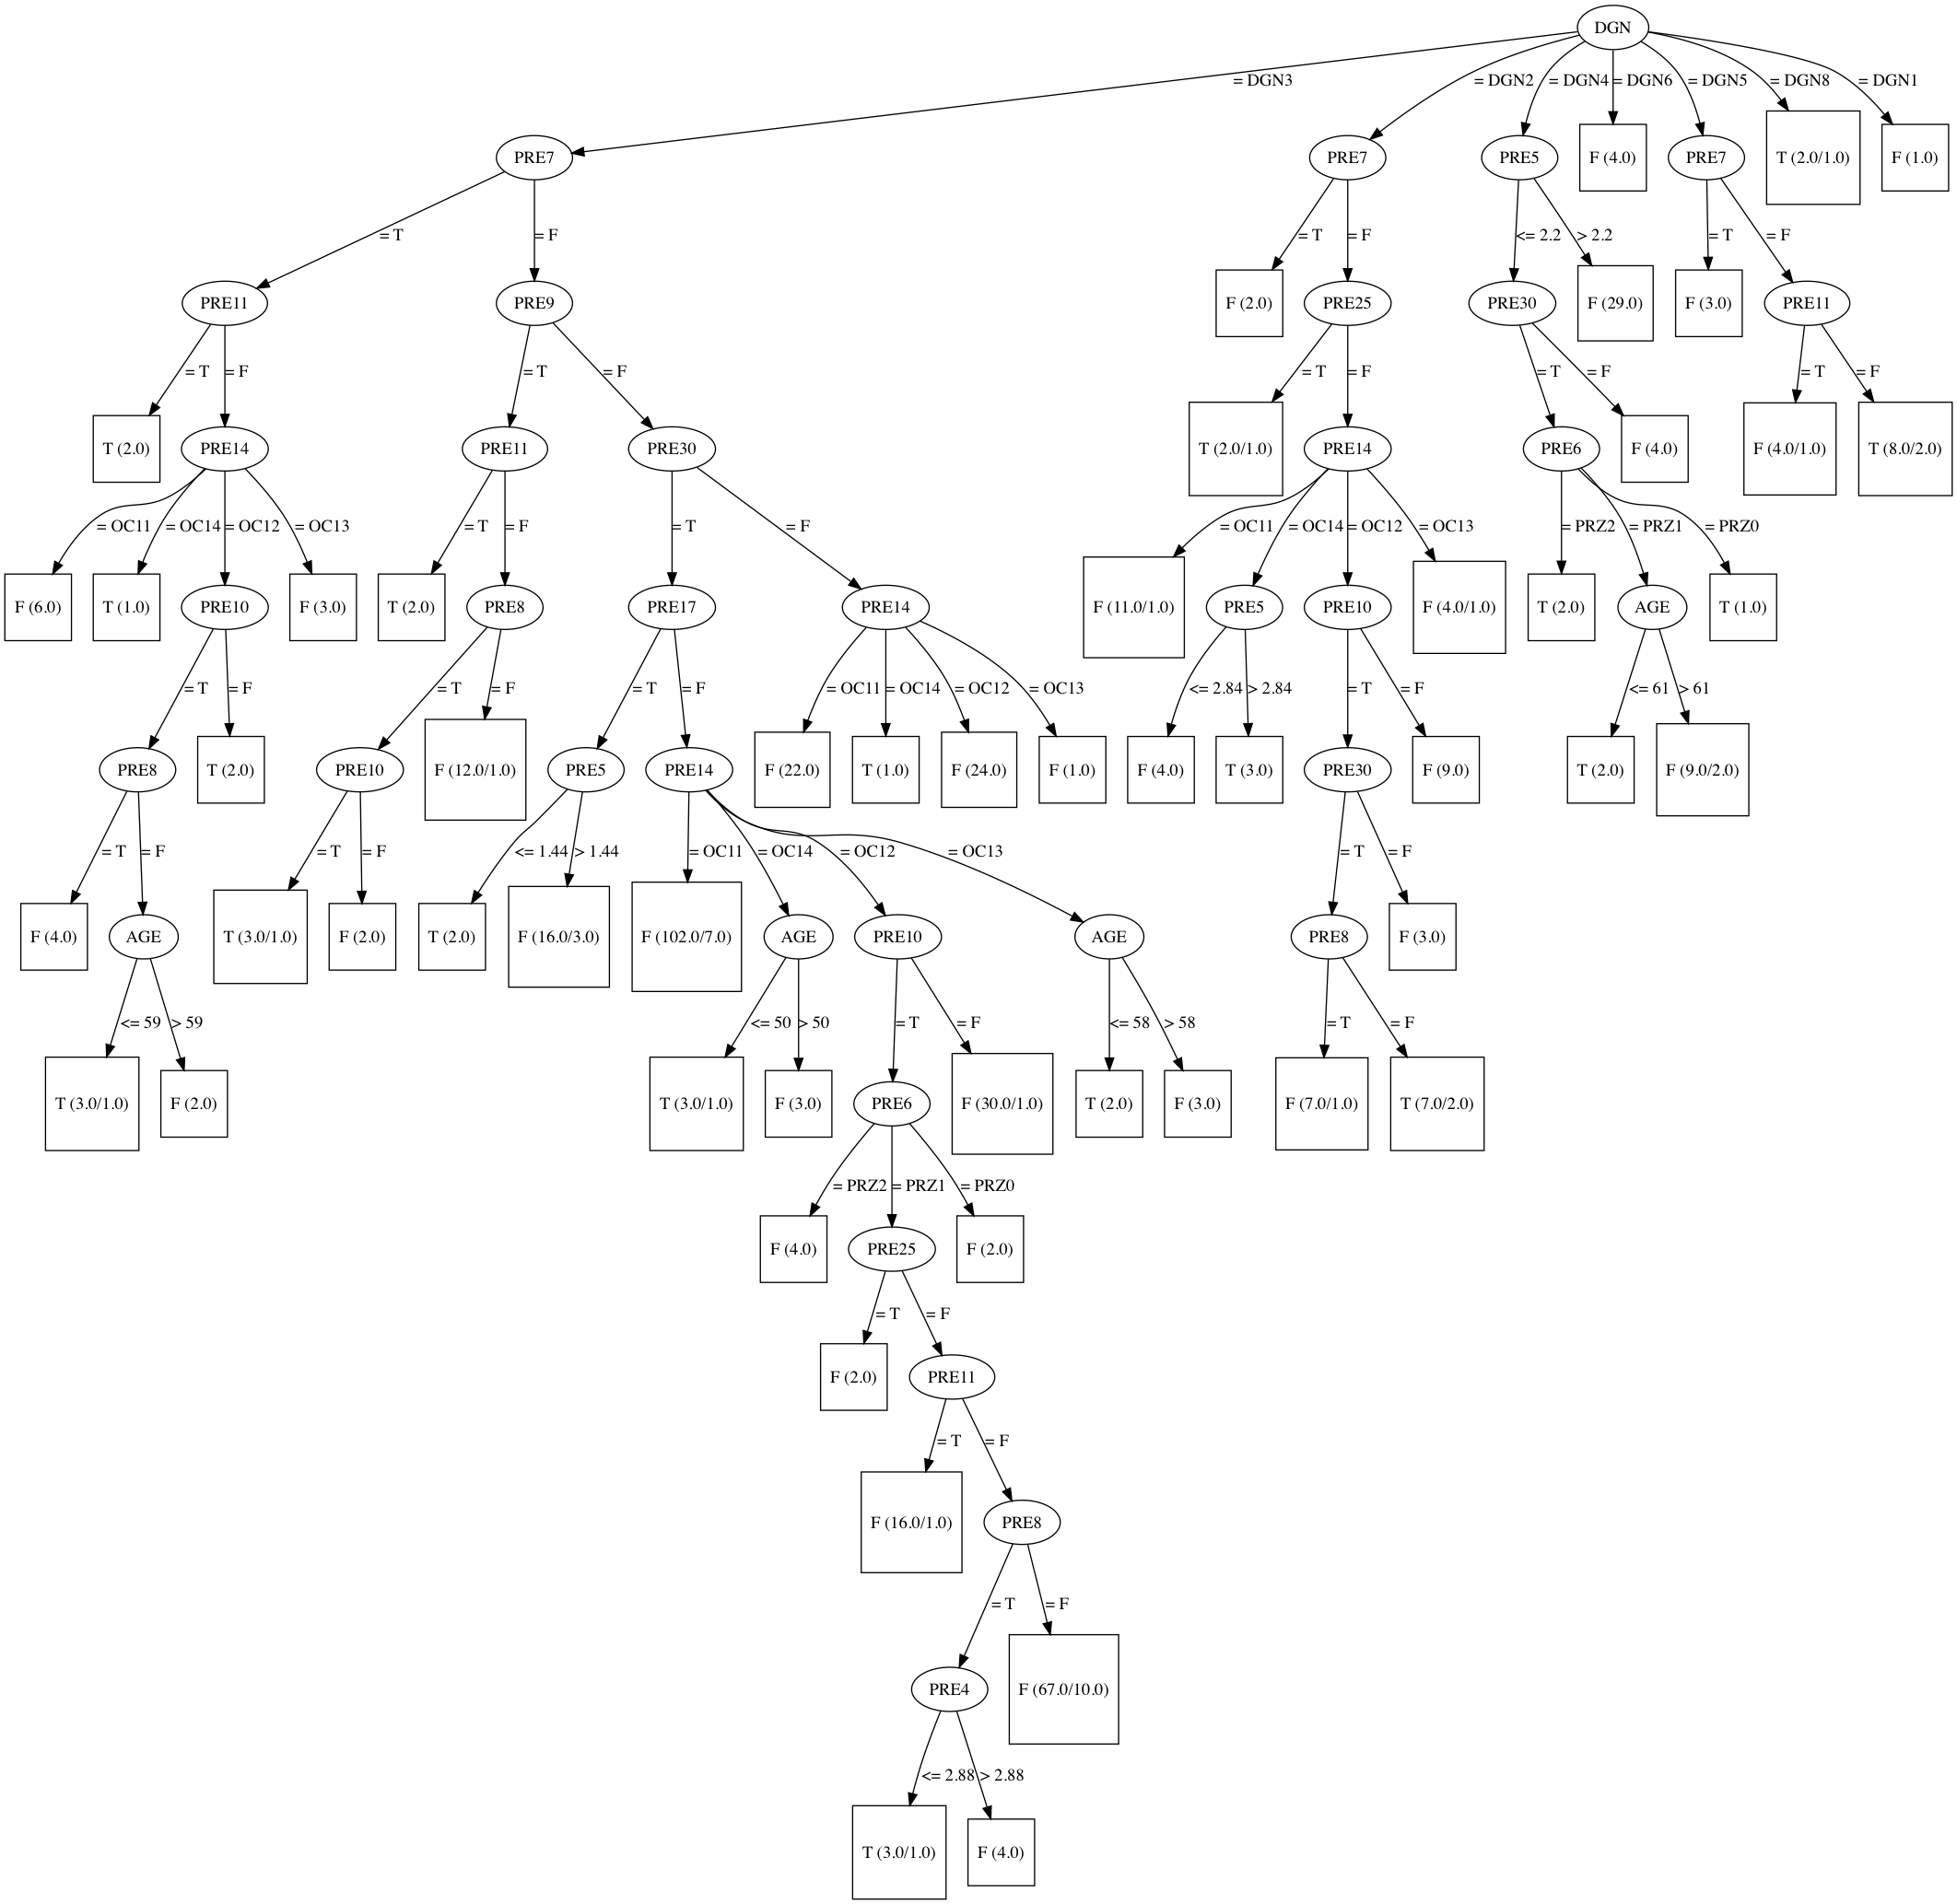
\includegraphics[width=\textwidth]{j48-tree-some}
			\end{center}
			\caption{Árbol de decisión generado a partir del algoritmo \emph{J48} tras eliminar los atributos no utilizados previamente.}
			\label{fig:j48-tree-some}
		\end{figure}


		\begin{table}[h]
			\begin{center}
				\begin{tabular}{r c c|c|l}
					& & \multicolumn{2}{ c }{Valor Real} \\ \cline{3-4}
					& & \multicolumn{1}{ |c| }{Positivo} & \multicolumn{1}{ |c| }{Negativo} & \multicolumn{1}{ l }{$p_j$}\\ \cline{2-4}
					\multicolumn{1}{  c  }{\multirow{2}{*}{Valor Predicho} } 	& \multicolumn{1}{ |c| }{Positivo} & $4$ & $18$ &  $0.1375$   \\ \cline{2-4}
					\multicolumn{1}{  c  }{}                        					& \multicolumn{1}{ |c| }{Negativo} & $22$  & $116$ & $0.8625$ \\ \cline{2-4}
					& \multicolumn{1}{ c }{$\pi_j$} & \multicolumn{1}{ c }{$0.1625$} & \multicolumn{1}{ c }{$0.8375$} & \multicolumn{1}{ l }{$N = 160$}
				\end{tabular}
			\end{center}
			\caption{Matriz de confusión del conjunto de datos entrenado por el algortimo \emph{J48}tras eliminar los atributos no utilizados previamente.}
			\label{table:confusion-matrix-j48-all}
		\end{table}

	\section{Habrá notado que cuando se usa algún atributo numérico, implícitamente se aplica una discretización al plantear las diferentes ramas del árbol a partir de él. ¿Por qué es más eficiente esta técnica que la aplicada en 2?}

		\paragraph{}


	\section{Plantee, entonces, una discretización basada en el punto anterior, aunque no resulte ser binaria, sino en tantos tramos como induzcan los valores usados al formar las ramas del árbol con J48 sin poda (Hold-Out). Introduzca este fichero de nuevo al algoritmo ID3. Compare los resultados con el J48 de 3}

		\paragraph{}



%-----------------------------
%	Bibliographic references
%-----------------------------
	\nocite{subject:taa}
	\nocite{github:ismtabo-treetograph}
  \bibliographystyle{acm}
  \bibliography{bib/misc}

\end{document}
